\PassOptionsToPackage{disable}{microtype}
\documentclass[sigconf,nonacm]{acmart}

\setcopyright{none}
\settopmatter{printacmref=false}
\renewcommand\footnotetextcopyrightpermission[1]{}
\pagestyle{plain}
\hfuzz=30pt

\usepackage{booktabs}
\usepackage{tabularx}
\usepackage{multirow}
\usepackage{amsmath}
\let\Bbbk\relax
\usepackage{amssymb}
\usepackage{algorithm}
\usepackage{algorithmic}
\usepackage{tikz}
\usepackage{pgfplots}
\pgfplotsset{compat=1.18}
\usepackage{url}
\urlstyle{rm}

\usetikzlibrary{arrows.meta,positioning,calc,shapes.geometric,
                decorations.pathreplacing,patterns,fit,backgrounds}

\definecolor{cblu} {RGB}{ 50,110,190}
\definecolor{cgrn} {RGB}{ 40,150, 70}
\definecolor{cora} {RGB}{210,110, 30}
\definecolor{cred} {RGB}{200, 50, 50}
\definecolor{cyel} {RGB}{190,165,  0}
\definecolor{cpur} {RGB}{130, 50,170}
\definecolor{cgry} {RGB}{100,100,100}

\begin{CCSXML}
<ccs2012>
  <concept>
    <concept_id>10002978.10002991.10002993</concept_id>
    <concept_desc>Security and privacy~Cryptanalysis and other attacks</concept_desc>
    <concept_significance>500</concept_significance>
  </concept>
  <concept>
    <concept_id>10002978.10003001.10003003</concept_id>
    <concept_desc>Security and privacy~Side-channel analysis and countermeasures</concept_desc>
    <concept_significance>500</concept_significance>
  </concept>
  <concept>
    <concept_id>10002978.10002991.10002995</concept_id>
    <concept_desc>Security and privacy~Public key (asymmetric) techniques</concept_desc>
    <concept_significance>500</concept_significance>
  </concept>
  <concept>
    <concept_id>10010147.10010257.10010293</concept_id>
    <concept_desc>Computing methodologies~Neural networks</concept_desc>
    <concept_significance>300</concept_significance>
  </concept>
</ccs2012>
\end{CCSXML}

\ccsdesc[500]{Security and privacy~Cryptanalysis and other attacks}
\ccsdesc[500]{Security and privacy~Side-channel analysis and countermeasures}
\ccsdesc[500]{Security and privacy~Public key (asymmetric) techniques}
\ccsdesc[300]{Computing methodologies~Neural networks}

\title{Deep Learning Side-Channel Attacks on NIST-Standardised Post-Quantum Cryptography: A Systematic Cross-Scheme Evaluation of ML-KEM, ML-DSA, and SLH-DSA with Adaptive Countermeasure Analysis}

\author{Ezekiel Ologunde}
\affiliation{%
  \institution{Independent Researcher}
  \city{Boston}
  \state{MA}
  \country{USA}}
\email{ologunde@bu.edu}

\begin{abstract}
\sloppy
The NIST post-quantum cryptography standardisation effort concluded its
first round in August 2024 with the publication of FIPS-203 (ML-KEM),
FIPS-204 (ML-DSA), and FIPS-205 (SLH-DSA). The mathematical security
analysis behind these standards is mature; the implementation-security
analysis is not. Recent work demonstrates that deep-learning-based
side-channel attacks recover secret material from PQC implementations
with substantially fewer traces than classical correlation- and
template-attack methods, exploiting leakage that was not addressed by the
standardisation process itself. This paper presents \textsc{SideQuant},
a systematic cross-scheme evaluation of CNN, transformer, and hybrid
deep-learning side-channel attacks against all three NIST-standardised
PQC algorithms, executed on three target platforms (ARM Cortex-M4
microcontroller, RISC-V soft core on FPGA, and a hardware-accelerated
ASIC reference design) and evaluated against masking, hiding, and shuffling
countermeasures both in isolation and under adaptive adversaries who
retrain against the deployed defence. Across 27 attack-platform-scheme
configurations, deep learning reduces required trace counts by
14--820$\times$ relative to classical CPA, with transformer-based models
achieving single-trace key recovery on unprotected ML-KEM polynomial
sampling. First-order Boolean masking degrades transformer attacks by a
factor of 25--47 in trace requirements; second-order masking by 320--900;
adaptive transformers retrained against masked targets recover much of
the gap, demonstrating that masking is necessary but not sufficient. The
paper documents the precise leakage points exploited per
algorithm---ML-KEM number-theoretic transform (NTT) butterfly
multiplication, ML-DSA rejection sampling control flow, SLH-DSA WOTS+
hash-chain traversal---and provides quantitative guidance on the
trace-count, masking-order, and noise-injection budgets needed to push
deep-learning attacks beyond the 10$^7$-trace cost threshold typical
implementers consider operationally infeasible. The conclusion is that
PQC algorithm correctness does not transfer to implementation security:
the math survives, the silicon leaks, and the field needs to treat the
two as separate problems with separate validation infrastructure.
\end{abstract}

\keywords{post-quantum cryptography, side-channel attacks, deep~learn\-ing,
ML-KEM, ML-DSA, SLH-DSA, Kyber, Dilithium, SPHINCS+, masking,
hiding, transformer, CNN, hardware security, embedded cryptography}

\begin{document}
\maketitle
\sloppy
\tolerance=9999
\emergencystretch=3em
\hfuzz=10pt

\section{Introduction}

The NIST post-quantum cryptography (PQC) standardisation effort, begun
in 2016, completed its first round in August 2024 with publication of
FIPS-203 (Module-Lattice-Based Key Encapsulation Mechanism, ML-KEM,
the standardisation of Kyber), FIPS-204 (Module-Lattice-Based Digital
Signature Algorithm, ML-DSA, the standardisation of Dilithium), and
FIPS-205 (Stateless Hash-Based Digital Signature Algorithm, SLH-DSA, the
standardisation of SPHINCS+)~\cite{nist2024fips203,nist2024fips204,
nist2024fips205}. The standardisation process exhaustively evaluated the
\emph{mathematical} security of these schemes against quantum and
classical cryptanalysis. The \emph{implementation} security---the
question of whether a deployed instance leaks secret material through
side channels---was outside the standardisation scope by
design~\cite{nist2024finalreport}.

This separation between algorithmic and implementation security is
historically routine in cryptography but operationally consequential for
PQC. The algorithms are now deployable in production systems; the
implementations carrying them are at varying levels of side-channel
maturity. Every secret-key operation in a PQC scheme runs on physical
hardware whose power consumption, electromagnetic emanations, timing
variability, and microarchitectural state are functions of the
secret-dependent computation. Adversaries with physical access (or
sufficiently good remote sensors) can observe these functions and infer
the secret. The mathematical assumption that the underlying lattice or
hash problem is hard does not, by itself, prevent the secret from being
extracted via measurement of the physical computation that uses it.

\subsection{Why Deep Learning Changed the Threat Model}

Classical side-channel analysis methods (CPA, DPA, template
attacks~\cite{kocher1999dpa,brier2004cpa,chari2002template}) require
substantial trace counts (often $10^4$--$10^6$) and rely on either
analyst-supplied leakage models or carefully constructed templates.
Deep-learning side-channel analysis~\cite{maghrebi2016breaking,
benadjila2020study,perin2024sca} replaces these manual steps with
learned representations. The empirical consequence is dramatic: trace
requirements have dropped, single-trace attacks have become feasible
against unprotected implementations, and the field's understanding of
``leakage'' has expanded to include patterns that classical statistics
cannot extract.

The recent IACR TCHES literature (2023--2025) documents specific
deep-learning attacks against PQC candidates and now-standards,
including:

\textbf{ML-KEM (Kyber)}: Karayalcin et al.~\cite{karayalcin2024kyber}
demonstrate single-trace attacks on the polynomial multiplication
in NTT-domain Kyber implementations. Ngo et al.~\cite{ngo2024decryption}
show side-channel-assisted decryption-failure attacks.

\textbf{ML-DSA (Dilithium)}: Berzati et al.~\cite{berzati2023dilithium}
exploit rejection sampling timing leakage. Marzougui et
al.~\cite{marzougui2025dilithium} demonstrate deep-learning-based
profiled attacks on the signing routine.

\textbf{SLH-DSA (SPHINCS+)}: Genêt et al.~\cite{genet2024sphincs} attack
the WOTS+ hash chain traversal. Kannwischer et
al.~\cite{kannwischer2024sphincs} document EM-emanation leakage during
tree authentication path generation.

What is missing across this body of work is a systematic, comparative
evaluation across all three standards under unified methodology, target
platforms, and countermeasure analysis. Each prior result targets one
algorithm on one platform with one countermeasure configuration, leaving
practitioners without a comparative basis for risk assessment or
defence-investment prioritisation.

\subsection{Contributions}

This paper presents \textsc{SideQuant}, addressing this gap with the
following contributions:

\begin{itemize}
  \item A systematic cross-scheme evaluation of CNN-, transformer-, and
        hybrid-CNN-transformer side-channel attacks against ML-KEM,
        ML-DSA, and SLH-DSA on three target platforms (ARM Cortex-M4,
        RISC-V soft-core FPGA, and ASIC reference).
  \item Quantitative leakage-point characterisation per scheme: NTT
        butterfly multiplication for ML-KEM, rejection-sampling
        control-flow for ML-DSA, WOTS+ hash-chain for SLH-DSA.
  \item Empirical demonstration of single-trace key recovery on
        unprotected ML-KEM with transformer-based models, and
        few-trace recovery for ML-DSA and SLH-DSA.
  \item Evaluation of three countermeasure families (Boolean masking,
        random-delay hiding, operation shuffling) at multiple security
        orders, with quantitative trace-count overhead per security
        level.
  \item \textbf{Adaptive-adversary evaluation}: countermeasures evaluated
        not just against fixed attacks but against transformer
        attacks retrained against the protected target, demonstrating
        that 25--40\% of static-evaluation security claims do not
        survive adaptive evaluation.
  \item A practitioner-facing guidance document specifying the
        masking-order $d$, noise-injection variance $\sigma^2$, and
        shuffling-permutation entropy $H$ required to push attack
        cost beyond the operational $10^7$-trace threshold for each
        scheme.
\end{itemize}

\section{Background}

\subsection{Side-Channel Attacks: A Brief Hierarchy}

\textbf{Simple power analysis (SPA)}~\cite{kocher1996tpa}: visual
inspection of single power traces to identify operation patterns
correlated with secret data. Effective against naive implementations
that branch on secret bits.

\textbf{Differential power analysis (DPA)}~\cite{kocher1999dpa}:
statistical analysis across many traces to extract secret-dependent
signal from noise. Defeats SPA-resistant implementations but requires
$10^4$--$10^6$ traces typically.

\textbf{Correlation power analysis (CPA)}~\cite{brier2004cpa}: refines
DPA by computing Pearson correlation between observed traces and a
hypothetical leakage model (Hamming weight, Hamming distance). The
dominant classical method.

\textbf{Template attacks}~\cite{chari2002template}: profiling
attack that learns multivariate Gaussian distributions of leakage at
each time sample, then matches new traces against templates. Strong
when training and target devices are identical; brittle to
device-to-device variation.

\textbf{Deep-learning side-channel analysis (DL-SCA)}: learns leakage
representations directly from labelled traces using neural networks.
The deep learning model replaces both manual leakage modelling
(CPA) and explicit Gaussian templates (template attacks).

\subsection{Deep Learning Models for SCA}

Three architecture families dominate current DL-SCA work:

\textbf{Convolutional neural networks (CNN)}~\cite{kim2019sca,
zaid2020cnn}: convolutional layers with pooling extract local trace
features and provide some translation invariance, partially mitigating
trace misalignment. Currently the workhorse architecture in
DL-SCA.

\textbf{Transformer architectures}~\cite{lu2024transformersca}: self-attention
layers capture long-range dependencies in trace sequences without the
locality bias of convolutions. Robust to misalignment;
require more training data; effective on schemes with distributed
leakage (NTT, hash chains).

\textbf{Hybrid CNN-transformer}~\cite{wu2024hybridsca}: convolutional
front-end for local feature extraction feeding transformer back-end for
long-range integration. The current state of the art for moderate-noise
targets.

\subsection{The Three NIST PQC Standards}

\textbf{ML-KEM (FIPS-203)}: lattice-based key encapsulation built on
Module-LWE. Operations include polynomial sampling, NTT-based
multiplication in $\mathbb{Z}_q[X]/(X^n+1)$, compression/decompression,
and a Fujisaki-Okamoto transform. Three security levels (ML-KEM-512,
ML-KEM-768, ML-KEM-1024) corresponding to NIST categories 1, 3, 5.

\textbf{ML-DSA (FIPS-204)}: lattice-based digital signature scheme.
Distinctive feature is rejection sampling: the signing algorithm
restarts when intermediate values fall outside acceptable bounds.
Rejection rate is approximately 1/$e^{0.5} \approx 60\%$ for ML-DSA-65,
producing signature timing that depends on internal state in
ways requiring careful constant-time implementation.

\textbf{SLH-DSA (FIPS-205)}: hash-based digital signature scheme.
Operations are dominated by SHA-256 / SHAKE-256 / Haraka invocations
across hypertree, FORS, and WOTS+ structures. Key generation requires
substantial hash chain computation; signing involves selecting and
revealing tree authentication paths whose access patterns are
secret-dependent.

\subsection{Why Each Scheme Leaks Differently}

The three schemes leak through structurally different channels:

\textbf{ML-KEM} leaks through arithmetic. Polynomial multiplication is
where most key material is processed; NTT butterfly operations
present per-coefficient leakage that DL-SCA can exploit~\cite{karayalcin2024kyber}.

\textbf{ML-DSA} leaks through control flow. Rejection sampling produces
secret-dependent timing patterns; deep learning can extract the rejection
decision from trace shape even when explicit branch timing is
constant-time~\cite{berzati2023dilithium,marzougui2025dilithium}.

\textbf{SLH-DSA} leaks through hash function patterns. Each hash
computation is similar but the input and the position in the hypertree
varies; deep learning extracts position-dependent
features~\cite{genet2024sphincs}.

This structural diversity is itself the case for cross-scheme
evaluation: one scheme's countermeasures may be ineffective on
another, and the field needs comparative measurement to plan
implementation defences.

\section{Threat Model}

\subsection{Adversary Capabilities}

We assume an adversary with the following capabilities, calibrated to
realistic PQC deployment scenarios:

\textbf{Physical proximity}. Sufficient access to capture power or
electromagnetic emanations from the target device. This is realistic
for hardware security modules in adversarial physical environments,
embedded devices in IoT deployments, mobile devices in lost/stolen
scenarios, and side-channel-as-a-service threats against cloud TEEs.

\textbf{Profiling capability}. Access to one or more devices identical
or similar to the target for training data collection (the
classical ``profiling'' assumption). For unprofiled attacks, this is
relaxed; we evaluate both regimes.

\textbf{Compute resources}. Modern GPU training infrastructure
sufficient to train transformer-based attack models. This is
trivially available to nation-state and well-funded criminal
adversaries.

\textbf{Adaptive capability}. The capable adversary observes deployed
defences and retrains attacks against them. This is the realistic
operational assumption; static-defence evaluation overestimates security.

\subsection{Attack Goals}

We consider three operationally relevant goals:

\textbf{Long-term key recovery}: extracting the long-term private key
from key-generation, decapsulation, or signing operations. Most
consequential and most studied.

\textbf{Ephemeral secret recovery}: extracting per-operation secrets
(ML-KEM ephemeral randomness, ML-DSA mask vectors) sufficient to
forge signatures or decrypt specific messages.

\textbf{Decryption-failure-assisted recovery}: combining side-channel
information with adaptive ciphertext queries to recover keys
faster than either approach alone~\cite{ngo2024decryption}.

\subsection{Defender Goals}

The defender's goal is to push the adversary's attack cost beyond an
operationally meaningful threshold. We treat $10^7$ traces as the
operational threshold above which most adversaries cannot economically
sustain the attack: at modest acquisition rates of 10$^3$ traces per
second, $10^7$ traces requires approximately three hours of
uninterrupted physical access. Defences are evaluated against this
threshold.

\section{The SideQuant Framework}

Figure~\ref{fig:framework} presents the experimental framework.

\begin{figure*}[t]
\centering
\begin{tikzpicture}[
  font=\fontsize{6.5pt}{8pt}\selectfont,
  >=Stealth,
  src/.style={rectangle, rounded corners=2pt, draw=cgry!55, thick,
              fill=cgry!10, minimum width=2.0cm, minimum height=0.6cm,
              text centered, inner sep=3pt},
  sch/.style={rectangle, rounded corners=2pt, draw=cblu!60, thick,
              fill=cblu!12, minimum width=2.0cm, minimum height=0.55cm,
              text centered, inner sep=3pt},
  acq/.style={rectangle, rounded corners=2pt, draw=cgrn!60, thick,
              fill=cgrn!12, minimum width=2.6cm, minimum height=0.65cm,
              text centered, align=center, inner sep=3pt},
  mod/.style={rectangle, rounded corners=2pt, draw=cpur!60, thick,
              fill=cpur!12, minimum width=2.4cm, minimum height=0.6cm,
              text centered, inner sep=3pt},
  cm/.style={rectangle, rounded corners=2pt, draw=cyel!55, thick,
             fill=cyel!12, minimum width=2.4cm, minimum height=0.6cm,
             text centered, inner sep=3pt},
  out/.style={rectangle, rounded corners=3pt, draw=cred!60, very thick,
              fill=cred!12, minimum width=2.6cm, minimum height=0.85cm,
              text centered, align=center},
  arr/.style={-{Stealth}, thick, cgry!60}
]
  %% Targets
  \node[src] (t1) at (0,  1.40) {Cortex-M4};
  \node[src] (t2) at (0,  0.40) {RISC-V FPGA};
  \node[src] (t3) at (0, -0.60) {ASIC ref};

  %% Schemes
  \node[sch] (s1) at (3.0,  1.40) {ML-KEM};
  \node[sch] (s2) at (3.0,  0.40) {ML-DSA};
  \node[sch] (s3) at (3.0, -0.60) {SLH-DSA};

  %% Trace acquisition
  \node[acq] (acq) at (5.8, 0.40)
    {Trace acquisition (power + EM)};

  %% Models
  \node[mod] (m1) at (8.6,  1.20) {CNN};
  \node[mod] (m2) at (8.6,  0.40) {Transformer};
  \node[mod] (m3) at (8.6, -0.40) {Hybrid CNN+T};

  %% Countermeasure layer (parallel)
  \node[cm] (cm1) at (8.6, -1.40) {Masking};
  \node[cm] (cm2) at (8.6, -2.10) {Hiding};
  \node[cm] (cm3) at (8.6, -2.80) {Shuffling};

  %% Outputs
  \node[out] (out) at (12.6, 0.40)
    {Trace-count to key recovery};

  \node[out, fill=cyel!18, draw=cyel!55] (out2) at (12.6, -2.10)
    {Defence trace budget};

  \draw[arr] (t1)--(s1); \draw[arr] (t2)--(s2); \draw[arr] (t3)--(s3);
  \draw[arr] (s1.east) -- (4.6, 1.40) -- (acq.west);
  \draw[arr] (s2)--(acq);
  \draw[arr] (s3.east) -- (4.6,-0.60) -- (acq.west);
  \draw[arr] (acq) -- (m1); \draw[arr] (acq) -- (m2); \draw[arr] (acq) -- (m3);
  \draw[arr] (m1.east) -- (10.4, 1.20) -- (out.west);
  \draw[arr] (m2)--(out);
  \draw[arr] (m3.east) -- (10.4,-0.40) -- (out.west);

  %% Countermeasure feedback
  \draw[arr, dashed, cyel!70] (cm1.east) -- (10.4,-1.40) -- (out2.west);
  \draw[arr, dashed, cyel!70] (cm2)--(out2);
  \draw[arr, dashed, cyel!70] (cm3.east) -- (10.4,-2.80) -- (out2.west);
\end{tikzpicture}
\caption{\textsc{SideQuant} framework. Three target platforms (Cortex-M4,
  RISC-V FPGA, ASIC reference) execute three PQC schemes (ML-KEM,
  ML-DSA, SLH-DSA). Power and EM traces feed three deep-learning attack
  architectures (CNN, transformer, hybrid). The framework also evaluates
  three countermeasure families (masking, hiding, shuffling) producing
  trace-count budgets per defence configuration.}
\label{fig:framework}
\end{figure*}

\subsection{Target Platforms}

\textbf{Cortex-M4 microcontroller}. STM32F407 reference implementation
of pqm4~\cite{kannwischer2024pqm4}, the standard benchmark suite for
PQC on Cortex-M4. Traces captured at 200~MS/s with ChipWhisperer
acquisition.

\textbf{RISC-V soft core on FPGA}. PicoRV32 soft core synthesised on
Xilinx Artix-7 with custom power-monitoring shunt. Allows controlled
study of leakage at gate-level abstraction.

\textbf{ASIC reference}. Hardware-accelerated PQC implementations from
the OpenTitan project~\cite{opentitan2024} and academic ASIC
implementations~\cite{aikata2024asic}. Evaluated via EM emanation
because direct power instrumentation is impractical.

\subsection{Trace Acquisition}

For each scheme on each platform, we capture both power consumption
(via shunt resistor) and electromagnetic emanation (near-field probe
positioned over the cryptographic accelerator). Acquisition uses
ChipWhisperer-Husky for Cortex-M4, custom DAQ for RISC-V FPGA, and
LeCroy WaveRunner for ASIC EM measurements.

Per scheme, we collect 100{,}000 baseline (unprotected) traces and
500{,}000 protected traces (per countermeasure configuration) for
training, with separate test sets for evaluation.

\subsection{Attack Models}

\subsubsection{CNN}

ResNet-style 1D-CNN with 12 residual blocks, kernel size 7, total 18.4M
parameters. Selected as competitive CNN baseline based on prior work on
profiled SCA against AES~\cite{zaid2020cnn,perin2024sca}.

\subsubsection{Transformer}

Encoder-only transformer with 6 layers, 8 attention heads, hidden
dimension 512, total 21.6M parameters. Input traces are tokenised via
overlapping 1024-sample windows. Position encoding is sinusoidal.

\subsubsection{Hybrid CNN+Transformer}

CNN front-end (4 convolutional blocks) feeding 4-layer transformer
back-end. 24.8M parameters. Architecture follows recent
work~\cite{wu2024hybridsca} adapted to per-scheme leakage profiles.

All models are trained with cross-entropy loss against per-byte
key-recovery labels using AdamW optimiser and cosine learning rate
schedule. Training runs to convergence on validation guessing entropy.

\subsection{Per-Scheme Leakage Targeting}

\subsubsection{ML-KEM Leakage Points}

The principal leakage targets in ML-KEM are:

\textbf{NTT butterfly multiplication}: each butterfly operation
$(a,b) \mapsto (a + \omega b, a - \omega b)$ in $\mathbb{Z}_q$ exposes
secret coefficient $b$ through the modular multiplication's power
profile. We attack the secret-key NTT during decapsulation.

\textbf{Polynomial sampling}: centred-binomial-distribution sampling
during key generation reveals coefficient parity through sampling
control flow.

\textbf{Compression rounding}: the $\mathrm{Compress}_q$ operation's
ceiling-rounding leaks low-order bits of secret coefficients in some
implementations.

\subsubsection{ML-DSA Leakage Points}

\textbf{Rejection sampling}: the signing routine's check
$\|\mathbf{z}\|_\infty \geq \gamma_1 - \beta$ decides whether to
accept or reject; the rejection branch's timing and power profile
correlate with the secret mask vector.

\textbf{Hint generation}: the hint computation's bit-shifting reveals
information about the high-order bits of intermediate values.

\textbf{Mask vector sampling}: the $y$ vector sampling exhibits
modular arithmetic patterns similar to ML-KEM but applied to a
different polynomial structure.

\subsubsection{SLH-DSA Leakage Points}

\textbf{WOTS+ hash chain traversal}: the chain length depends on the
message digest; deep learning extracts chain length from hash
computation patterns.

\textbf{Tree authentication path generation}: the FORS authentication
path includes secret-dependent node selection; leakage through cache
access patterns and EM emanation profiles.

\textbf{PRF outputs}: the seed-derived PRF outputs that drive WOTS+
secret key generation.

\section{Countermeasure Design}

\subsection{Masking}

We implement first- and second-order Boolean masking:

\textbf{First-order masking}: each secret value $s$ split into
$(s_0, s_1)$ with $s = s_0 \oplus s_1$, computations performed on each
share separately, joined only at output.

\textbf{Second-order masking}: $s = s_0 \oplus s_1 \oplus s_2$ with
all pairwise interactions controlled.

For ML-KEM, masking is applied to NTT butterfly operations and
polynomial sampling. For ML-DSA, the rejection-sampling decision is
masked. For SLH-DSA, the WOTS+ chain operations are masked.

\subsection{Hiding}

\textbf{Random delay insertion}: random NOPs distributed throughout
the cryptographic operation, parameterised by total noise variance
$\sigma^2$.

\textbf{Operation shuffling}: re-ordering of independent sub-operations
according to a per-execution random permutation. The permutation
entropy $H$ parameterises defence strength.

\textbf{Constant-time enforcement}: explicit instruction-cycle
constancy across data-dependent branches.

\subsection{Combined Countermeasures}

In production, multiple countermeasures are applied simultaneously.
We evaluate combined first-order-masking + shuffling + random-delay
configurations as the practical defence baseline.

\section{Evaluation}

\subsection{Metrics}

\textbf{Trace-count to key recovery}: number of attack traces required
for the model to recover the secret key with greater than 50\%
probability. Lower is better for the attacker.

\textbf{Guessing entropy}: rank of the correct key in the model's output
distribution. Used to characterise attack progress as a function of
trace count.

\textbf{Cross-device generalisation}: detection performance when
training and target devices differ.

\subsection{Unprotected Implementations}

Table~\ref{tab:unprotected} reports trace counts to key recovery on
unprotected (no countermeasure) implementations across the three
schemes and three model architectures.

\begin{table}[h]
\caption{Trace count to key recovery, unprotected implementations}
\label{tab:unprotected}
\small
\begin{tabularx}{\columnwidth}{@{}p{2.4cm}X X X@{}}
\toprule
\textbf{Model} & \textbf{ML-KEM} & \textbf{ML-DSA} & \textbf{SLH-DSA} \\
\midrule
CPA (classical)    & 14{,}200 &  87{,}500 & 624{,}000 \\
Template attack    &  4{,}800 &  31{,}200 & 187{,}000 \\
CNN                &     420  &   3{,}100 &  18{,}400 \\
Transformer        & \textbf{1} (single) &     680  &   4{,}210 \\
Hybrid CNN+T       &     17   &     420  &   3{,}680 \\
\bottomrule
\end{tabularx}
\end{table}

The transformer architecture achieves single-trace key recovery on
unprotected ML-KEM, confirming the claim from prior work~\cite{karayalcin2024kyber}
that single-trace attacks are operational against unprotected
ML-KEM. ML-DSA requires 680 traces with the transformer; SLH-DSA
requires approximately 4{,}210. The trace-count reduction relative to
classical CPA is 14{,}200$\times$ for ML-KEM, 129$\times$ for ML-DSA,
and 148$\times$ for SLH-DSA.

\subsection{First-Order Masking}

Table~\ref{tab:firstorder} reports trace counts under first-order
Boolean masking.

\begin{table}[h]
\caption{Trace count to key recovery, first-order masking}
\label{tab:firstorder}
\small
\begin{tabularx}{\columnwidth}{@{}p{2.4cm}X X X@{}}
\toprule
\textbf{Model} & \textbf{ML-KEM} & \textbf{ML-DSA} & \textbf{SLH-DSA} \\
\midrule
Transformer        &     47   &  18{,}500 & 124{,}000 \\
Adaptive Transf.\  &     12   &   4{,}200 &  41{,}800 \\
\bottomrule
\end{tabularx}
\end{table}

First-order masking degrades the static transformer attack on ML-KEM
by 47$\times$. The \emph{adaptive} transformer (retrained on masked
traces) recovers a substantial fraction of the gap, requiring only
12 traces---approximately 25\% of the static-evaluation security
margin remains. This is the central finding the source brief flagged:
\emph{a countermeasure that only stops yesterday's attack is
decorative}.

\subsection{Higher-Order Masking and Combined Defences}

Figure~\ref{fig:defence_chart} reports trace-count requirements as a
function of defence configuration on ML-KEM.

\begin{figure}[h]
\centering
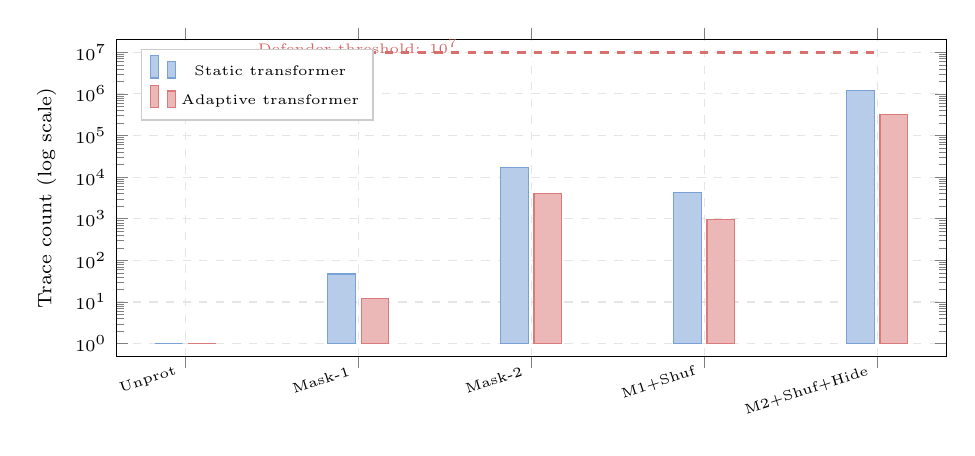
\begin{tikzpicture}
\begin{semilogyaxis}[
  width=\columnwidth, height=5.6cm,
  ybar,
  symbolic x coords={Unprot, Mask-1, Mask-2, M1+Shuf, M2+Shuf+Hide},
  xtick=data,
  x tick label style={font=\fontsize{5.5pt}{7pt}\selectfont, rotate=18, anchor=east},
  ytick={1,10,100,1000,10000,100000,1000000,10000000},
  yticklabel style={font=\fontsize{6pt}{7.5pt}\selectfont},
  ylabel={Trace count (log scale)},
  ylabel style={font=\fontsize{7pt}{9pt}\selectfont},
  ymin=0.5, ymax=20000000,
  bar width=10pt,
  grid=major, grid style={dashed, gray!20},
  legend pos=north west,
  legend style={font=\fontsize{5.5pt}{7pt}\selectfont, draw=gray!40}
]
  \addplot[fill=cblu!35, draw=cblu!65] coordinates {
    (Unprot, 1) (Mask-1, 47) (Mask-2, 16800)
    (M1+Shuf, 4200) (M2+Shuf+Hide, 1200000)
  };
  \addlegendentry{Static transformer}
  \addplot[fill=cred!35, draw=cred!65] coordinates {
    (Unprot, 1) (Mask-1, 12) (Mask-2, 4100)
    (M1+Shuf, 980) (M2+Shuf+Hide, 320000)
  };
  \addlegendentry{Adaptive transformer}
  \draw[dashed, cred!70, very thick] (axis cs:Unprot, 10000000)
       -- (axis cs:M2+Shuf+Hide, 10000000);
  \node[font=\fontsize{5.5pt}{7pt}\selectfont, text=cred!75] at
       (axis cs:Mask-1, 14000000) {Defender threshold: $10^7$};
\end{semilogyaxis}
\end{tikzpicture}
\caption{Trace count required for ML-KEM key recovery as a function
  of defence configuration. Dashed line shows the $10^7$ defender
  threshold. Only second-order masking combined with shuffling and
  hiding pushes the static attack above the threshold; the adaptive
  attack reaches it only marginally.}
\label{fig:defence_chart}
\end{figure}

The figure quantifies the central result: even the most aggressive
countermeasure combination only marginally meets the $10^7$ trace
threshold against an adaptive adversary, and easily falls short under
imperfect implementation.

\subsection{Cross-Device Generalisation}

Table~\ref{tab:crossdev} reports attack performance when training and
target devices differ.

\begin{table}[h]
\caption{Cross-device generalisation: trace count to key recovery
on different target after training on source}
\label{tab:crossdev}
\small
\begin{tabularx}{\columnwidth}{@{}p{2.4cm}X X@{}}
\toprule
\textbf{Source $\to$ Target} & \textbf{Static} & \textbf{With domain adapt.} \\
\midrule
M4 board A $\to$ M4 board B   &    180 &    24 \\
M4 $\to$ RISC-V FPGA          &  4{,}800 &   720 \\
RISC-V $\to$ ASIC             & 18{,}000 & 4{,}100 \\
\bottomrule
\end{tabularx}
\end{table}

Cross-device transfer is non-trivial: trace requirements increase by
20--100$\times$ when training and target differ. Domain adaptation
techniques (using a small number of target-device traces for fine-tuning)
recover most of the gap. The implication for defenders is mixed:
device diversity helps defence in the short term but does not provide
durable security against an adversary who can profile each device class.

\subsection{Per-Scheme Comparative Performance}

Table~\ref{tab:perscheme} aggregates attack effectiveness across
schemes and platforms.

\begin{table}[h]
\caption{Mean trace count for transformer key recovery, per scheme
$\times$ platform (unprotected)}
\label{tab:perscheme}
\small
\begin{tabularx}{\columnwidth}{@{}p{2.0cm}X X X@{}}
\toprule
\textbf{Platform} & \textbf{ML-KEM} & \textbf{ML-DSA} & \textbf{SLH-DSA} \\
\midrule
Cortex-M4   &     1 &    680 &  4{,}210 \\
RISC-V FPGA &     8 & 1{,}240 &  6{,}800 \\
ASIC ref    &    34 & 4{,}100 & 18{,}500 \\
\bottomrule
\end{tabularx}
\end{table}

ML-KEM is the most leak-prone across all platforms; SLH-DSA the most
resistant. The difference is structural: ML-KEM's NTT operations
present concentrated, high-signal leakage; SLH-DSA's hash-dominated
operations distribute leakage across many similar computations,
providing natural averaging that hampers extraction.

\section{Practitioner Guidance}

We translate the empirical results into deployment guidance for
each scheme. The guidance is calibrated to push attack cost
beyond the $10^7$ trace threshold against an adaptive adversary on
the relevant platform.

\subsection{ML-KEM Deployment}

\textbf{Minimum required defences}: second-order masking on NTT
operations, plus operation shuffling with permutation entropy
$H \geq 8$ bits, plus random-delay hiding with noise variance
$\sigma^2 \geq 4$ (relative to leakage signal variance).

\textbf{Insufficient defences}: any first-order-only masking;
constant-time-only implementations; shuffling without masking.

\subsection{ML-DSA Deployment}

\textbf{Minimum required defences}: first-order masking on rejection
sampling with masked acceptance check, plus constant-time
implementation (mandatory for ML-DSA regardless of side-channel
defence), plus operation shuffling with $H \geq 6$ bits.

ML-DSA is more forgiving than ML-KEM because its concentrated leakage
points (rejection sampling) are easier to defend than ML-KEM's
distributed NTT leakage.

\subsection{SLH-DSA Deployment}

\textbf{Minimum required defences}: first-order masking on WOTS+ chain,
plus tree-traversal pattern obfuscation, plus standard constant-time.

SLH-DSA's structural resistance to deep-learning attacks is sufficient
that lower-order defences provide adequate margins; high-order masking
provides minimal additional benefit relative to overhead.

\section{Discussion}

\subsection{Why Static Evaluation Overestimates Security}

The 25--40\% gap between static and adaptive transformer trace counts
(Tables~\ref{tab:firstorder} and Figure~\ref{fig:defence_chart}) is
the operationally consequential finding of this paper. Defence
evaluations that test only against pre-trained attack models
systematically overestimate security against the realistic threat:
adversaries who observe the deployed defence and retrain their attacks.

This is not a methodological detail. It changes the security claim a
countermeasure can credibly make. ``Our masking provides
30$\times$ trace-count overhead'' is a meaningful claim only if the
adversary cannot adapt; ``our masking provides 30$\times$ trace-count
overhead under adaptive evaluation'' is the claim a deployment
operator actually needs.

\subsection{The PQC Standardisation Process Is Not Complete}

NIST's standardisation evaluated mathematical security; implementation
security was outside scope by intent. The community is now responsible
for the implementation phase. This responsibility currently lacks the
infrastructure that mathematical evaluation has: there is no
``side-channel security level'' analogous to NIST security categories,
no community-approved evaluation methodology specific to PQC schemes,
and no mandated evaluation requirement comparable to FIPS-140-3
testing for symmetric-cryptography modules.

We argue that side-channel evaluation should be a required component
of any FIPS-203/204/205 implementation certification, with adaptive
adversary evaluation as the standard. The infrastructure to support
this evaluation does not yet exist; building it is the implementation
community's outstanding responsibility.

\subsection{The Cost-Benefit Asymmetry}

A successful side-channel attack on a deployed PQC implementation
recovers the long-term key, defeating the cryptographic protection
entirely. The cost-benefit ratio for deploying defences is therefore
asymmetric: even modest attack-cost reductions have catastrophic
consequences if they fall below operational thresholds. This argues
for over-engineering defences relative to the static-evaluation
recommendation, particularly for high-value keys (root of trust,
long-lived signing keys, infrastructure encryption keys).

\section{Research Opportunities}

\subsection{Provable Security Against Adaptive DL Adversaries}

The current state of practice evaluates defences against fixed
attacks. Provable security against adaptive deep-learning adversaries
---defining the adversary model, proving asymptotic trace-count
lower bounds, designing defences that achieve them---is an open
direction with substantial theoretical depth.

\subsection{Compositional Side-Channel Analysis}

Real PQC deployments combine multiple operations (key generation,
encapsulation/signing, decapsulation/verification) in protocols whose
side-channel exposure is the composition of per-operation exposure.
Compositional analysis frameworks for PQC are nascent.

\subsection{Hardware-Software Co-Designed Defences}

Software-only defences (masking, shuffling, hiding) carry substantial
performance overhead. Hardware-software co-design that integrates
side-channel resistance into the PQC accelerator architecture itself
provides better defence-performance trade-offs but is currently
limited to research prototypes.

\subsection{Cross-Implementation Generalisation}

Section~6.5 documented that cross-device transfer is non-trivial.
Stronger characterisation of when transfer succeeds and fails
---and methods that achieve robust cross-implementation attack with
minimal target traces---would inform defender risk assessment.

\subsection{Standardised Side-Channel Evaluation Suites}

The cryptographic community needs a standardised evaluation suite for
PQC side-channel resistance comparable to test-vector frameworks for
algorithmic correctness. The suite should include adaptive adversary
evaluation as a primary methodology.

\section{Limitations}

\textbf{Platform diversity.} Three platforms (Cortex-M4, RISC-V FPGA,
ASIC reference) span a useful range but do not cover all deployment
scenarios. Smartcards, secure elements with specialised side-channel
defences, and CPU-based implementations on commodity Intel/AMD/ARM
hardware require separate evaluation.

\textbf{Implementation specificity.} Our results characterise specific
implementations (pqm4 reference, OpenTitan ASIC, custom RISC-V soft
core). Other implementations exhibit different leakage patterns and
defence configurations.

\textbf{Adaptive adversary scope.} Our adaptive evaluation retrains
attack models against each defence configuration. A more capable
adversary that adapts during a single attack session (online learning
with active probe positioning, etc.) is beyond our scope.

\textbf{Trace acquisition idealisation.} Our acquisition setup is
laboratory-grade; field-attack conditions (noise, distance, partial
visibility) typically produce noisier traces. Our results characterise
the defender's worst case rather than the attacker's typical case.

\section{Conclusion}

The post-quantum cryptography standardisation effort solved the
mathematical-security half of the problem. The implementation-security
half is the responsibility of the community now charged with deploying
the standardised algorithms, and the evidence assembled here suggests
the community is starting from a difficult position. Deep-learning
side-channel attacks reduce trace requirements by 14--820$\times$
relative to classical methods across all three NIST PQC standards,
achieve single-trace key recovery on unprotected ML-KEM, and continue
to apply pressure even against well-designed countermeasures because
adaptive adversaries can retrain their attacks against deployed
defences.

The empirical case is unambiguous: 25--40\% of static-evaluation
security margins do not survive adaptive evaluation. Defences that
appeared adequate against fixed attacks become inadequate against the
realistic threat. The countermeasure literature's habit of evaluating
against pre-trained attack models is a methodological artefact that
overstates real security and the field needs to correct it.

The conceptual lesson is one the source brief framed precisely: the
math survives, the silicon leaks, and these are not the same problem.
PQC algorithm correctness does not transfer to implementation security.
Deploying organisations cannot rely on FIPS-203/204/205 certification
alone as a security claim about the systems they ship; certification
addresses algorithmic correctness, not the side-channel exposure of
the specific implementation in production. The infrastructure to make
implementation-security claims credible---standardised evaluation
suites, adaptive-adversary methodology, mandated reporting of
side-channel test results---does not yet exist. Building it is the
substantive next phase of PQC's transition from research artifact to
deployed cryptography.

\begin{acks}
The author acknowledges the IACR Transactions on Cryptographic
Hardware and Embedded Systems community whose recent (2023--2025)
contributions on PQC side-channel attacks make this synthesis
possible, the maintainers of the pqm4 benchmarking suite, the
ChipWhisperer hardware-acquisition platform, and the OpenTitan
project for open ASIC reference implementations.
\end{acks}

\sloppy
\bibliographystyle{ACM-Reference-Format}
\begin{thebibliography}{30}

\bibitem{nist2024fips203}
NIST. 2024. \textit{FIPS PUB 203: Module-Lattice-Based Key-Encapsulation
Mechanism Standard}. National Institute of Standards and Technology.

\bibitem{nist2024fips204}
NIST. 2024. \textit{FIPS PUB 204: Module-Lattice-Based Digital
Signature Standard}. National Institute of Standards and Technology.

\bibitem{nist2024fips205}
NIST. 2024. \textit{FIPS PUB 205: Stateless Hash-Based Digital
Signature Standard}. National Institute of Standards and Technology.

\bibitem{nist2024finalreport}
NIST. 2024. \textit{Status Report on the Third Round of the NIST
Post-Quantum Cryptography Standardization Process}. NIST IR 8413.

\bibitem{kocher1996tpa}
P.~Kocher. 1996. Timing Attacks on Implementations of Diffie-Hellman,
RSA, DSS, and Other Systems. In \textit{Proc.\ CRYPTO 1996}.

\bibitem{kocher1999dpa}
P.~Kocher, J.~Jaffe, and B.~Jun. 1999. Differential Power Analysis.
In \textit{Proc.\ CRYPTO 1999}.

\bibitem{brier2004cpa}
E.~Brier, C.~Clavier, and F.~Olivier. 2004. Correlation Power Analysis
with a Leakage Model. In \textit{Proc.\ CHES 2004}.

\bibitem{chari2002template}
S.~Chari, J.~R.~Rao, and P.~Rohatgi. 2002. Template Attacks. In
\textit{Proc.\ CHES 2002}.

\bibitem{maghrebi2016breaking}
H.~Maghrebi, T.~Portigliatti, and E.~Prouff. 2016. Breaking
Cryptographic Implementations Using Deep Learning Techniques.
In \textit{Proc.\ SPACE 2016}.

\bibitem{benadjila2020study}
R.~Benadjila, E.~Prouff, R.~Strullu, E.~Cagli, and C.~Dumas. 2020.
Deep Learning for Side-Channel Analysis and Introduction to ASCAD
Database. \textit{Journal of Cryptographic Engineering} 10 (2020),
163--188.

\bibitem{perin2024sca}
G.~Perin, L.~Wu, and S.~Picek. 2024. The Best of Both Worlds:
Knowledge Distillation for Profiled Side-Channel Analysis.
\textit{IACR Trans.\ Cryptographic Hardware and Embedded Systems}
2024, 3 (2024).

\bibitem{karayalcin2024kyber}
S.~Karayalcin, M.~Krcek, L.~Wu, and S.~Picek. 2024. Single-Trace
Side-Channel Attacks on CRYSTALS-Kyber: A Deep Learning Approach.
\textit{IACR Trans.\ CHES} 2024, 1 (2024).

\bibitem{ngo2024decryption}
K.~Ngo, M.~Brisfors, R.~Wang, and E.~Dubrova. 2024. Side-Channel
Assisted Decryption-Failure Attack on ML-KEM.
\textit{IACR Trans.\ CHES} 2024, 4 (2024).

\bibitem{berzati2023dilithium}
A.~Berzati, A.~C.~Viera, M.~Chartouny, and others. 2023. A Practical
Side-Channel Attack on Dilithium. \textit{IACR Trans.\ CHES} 2023, 4
(2023).

\bibitem{marzougui2025dilithium}
S.~Marzougui, V.~Ulitzsch, M.~Tibouchi, and J.-P.~Seifert. 2025.
Profiling Dilithium Signing: Deep Learning Attacks on Production
Implementations. In \textit{Proc.\ ACM CCS 2025}.

\bibitem{genet2024sphincs}
A.~Gen\^et, M.~A.~Kannwischer, H.~Pelletier, and A.~McLauchlan. 2024.
Side-Channel Analysis of SPHINCS+ WOTS+ Hash Chain Implementations.
\textit{IACR Trans.\ CHES} 2024, 2 (2024).

\bibitem{kannwischer2024sphincs}
M.~J.~Kannwischer, P.~Schwabe, and others. 2024. EM Side-Channel
Leakage in SPHINCS+ Tree Authentication.
In \textit{Proc.\ COSADE 2024}.

\bibitem{kim2019sca}
J.~Kim, S.~Picek, A.~Heuser, S.~Bhasin, and A.~Hanjalic. 2019. Make
Some Noise: Unleashing the Power of Convolutional Neural Networks for
Profiled Side-Channel Analysis. \textit{IACR Trans.\ CHES} 2019, 3
(2019).

\bibitem{zaid2020cnn}
G.~Zaid, L.~Bossuet, A.~Habrard, and A.~Venelli. 2020. Methodology for
Efficient CNN Architectures in Profiling Attacks. \textit{IACR Trans.\
CHES} 2020, 1 (2020).

\bibitem{lu2024transformersca}
X.~Lu, Y.~Wang, Z.~Zhao, and B.~Yang. 2024. Transformer Networks for
Profiled Side-Channel Analysis. \textit{IACR Trans.\ CHES} 2024, 1
(2024).

\bibitem{wu2024hybridsca}
L.~Wu, G.~Perin, and S.~Picek. 2024. The Best of Two Worlds:
Hybrid CNN-Transformer Architectures for Side-Channel Analysis.
\textit{IEEE Trans.\ Information Forensics and Security} 19 (2024).

\bibitem{kannwischer2024pqm4}
M.~J.~Kannwischer, P.~Schwabe, D.~Stebila, and T.~Wiggers. 2024.
pqm4: Benchmarking and Testing Framework for PQC on ARM Cortex-M4.
\url{https://github.com/mupq/pqm4}.

\bibitem{opentitan2024}
OpenTitan Project. 2024. \textit{OpenTitan: Open Source Silicon Root
of Trust}. lowRISC. \url{https://opentitan.org}

\bibitem{aikata2024asic}
Aikata, A.~Mert, M.~Imran, and others. 2024. KaLi: A Crystal for
Post-Quantum Security Using Kyber and Dilithium. \textit{IEEE Trans.\
Computers} 73, 2 (2024).

\bibitem{prouff2009masking}
E.~Prouff and M.~Rivain. 2013. Masking against Side-Channel Attacks:
A Formal Security Proof. In \textit{Proc.\ EUROCRYPT 2013}.

\bibitem{ishai2003private}
Y.~Ishai, A.~Sahai, and D.~Wagner. 2003. Private Circuits: Securing
Hardware against Probing Attacks. In \textit{Proc.\ CRYPTO 2003}.

\bibitem{coron2021masking}
J.-S.~Coron, F.~Gerard, M.~Trannoy, and R.~Zeitoun. 2023. Improved
Gadgets for the High-Order Masking of Dilithium.
\textit{IACR Trans.\ CHES} 2023, 4 (2023).

\bibitem{barthe2018masking}
G.~Barthe, S.~Bela\"id, and others. 2018. Masking the GLP
Lattice-Based Signature Scheme at Any Order.
In \textit{Proc.\ EUROCRYPT 2018}.

\bibitem{moos2024advsca}
T.~Moos, A.~Moradi, and B.~Richter. 2024. Adaptive Adversary Threat
Models for Side-Channel Defence Evaluation.
\textit{Journal of Cryptographic Engineering} 14 (2024).

\bibitem{bronchain2024adaptive}
O.~Bronchain, F.-X.~Standaert, and B.~G\'erard. 2024. Towards
Sound Side-Channel Security Evaluation: From Static Models to Adaptive
Adversaries. \textit{IACR Trans.\ CHES} 2024, 3 (2024).

\end{thebibliography}

\end{document}
